\renewcommand*{\arraystretch}{1.1}

\subsection*{BI / read / 16}
\label{section:bi-read-16}

\noindent\begin{tabularx}{\queryCardWidth}{|>{\queryPropertyCell}p{\queryPropertyCellWidth}|X|}
	\hline
	query & BI / read / 16 \\ \hline
%
	title & Experts in social circle
 \\ \hline
%
	pattern & \hfill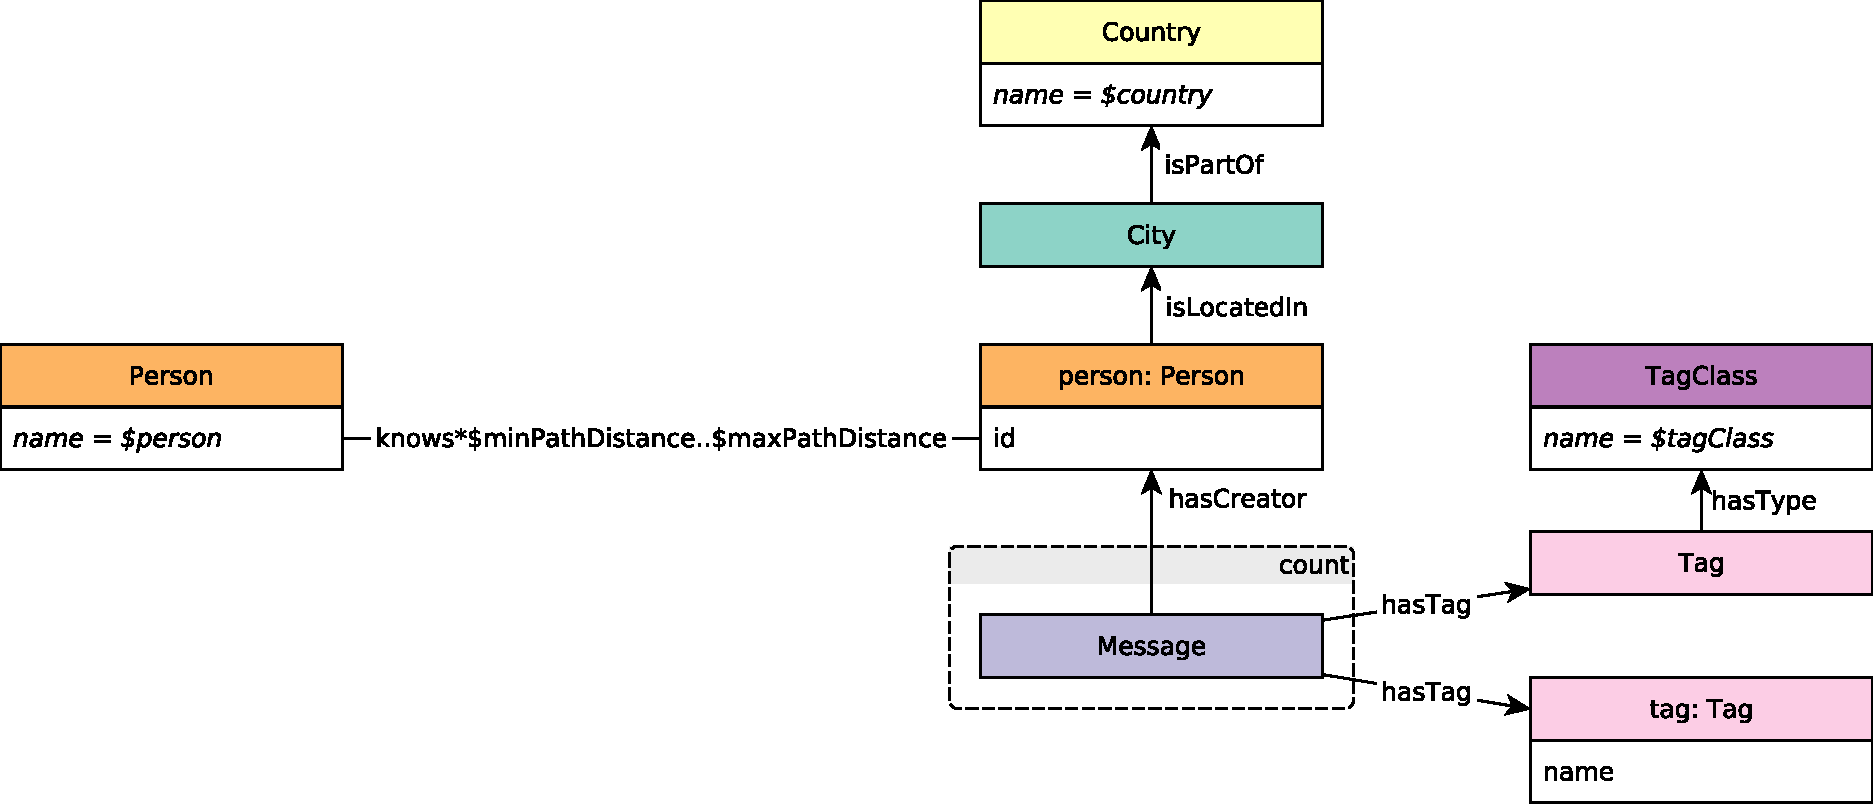
\includegraphics[scale=\patternscale,margin=0cm .2cm]{patterns/bi-read-16}\hfill\vadjust{} \\ \hline
%
	desc. & Given a Person, find all other Persons that live in a given country and
are connected to given person by a transitive path with length in range
{[}min, max{]} through the knows relation.

In the path, an edge can be only traversed once while nodes can be
traversed multiple times.

For each of these \emph{Persons}, retrieve all of their \emph{Messages}
(\emph{Posts} \& \emph{Comments}) that contain at least one \emph{Tag}
belonging to a given \emph{TagClass} (direct relation not transitive).
For each \emph{Message}, retrieve all of its \emph{Tags}.

Group the results by \emph{Persons} and \emph{Tags}, then count the
\emph{Messages} by a certain \emph{Person} having a certain \emph{Tag}.
 \\ \hline
%
	
		params &
		\innerCardVSpace{\begin{tabularx}{\attributeCardWidth}{|>{\paramNumberCell}c|>{\varNameCell}M|>{\typeCell}m{\typeWidth}|Y|} \hline
		$\mathsf{1}$ & person
 & String
 &  \\ \hline
		$\mathsf{2}$ & country
 & String
 &  \\ \hline
		$\mathsf{3}$ & tagClass
 & String
 &  \\ \hline
		$\mathsf{4}$ & minPathDistance
 & 32-bit Integer
 &  \\ \hline
		$\mathsf{5}$ & maxPathDistance
 & 32-bit Integer
 &  \\ \hline
		\end{tabularx}}\innerCardVSpace \\ \hline
	
%
	
		result &
		\innerCardVSpace{\begin{tabularx}{\attributeCardWidth}{|>{\resultNumberCell}c|>{\varNameCell}M|>{\typeCell}m{\typeWidth}|>{\resultOriginCell}c|Y|} \hline
		$\mathsf{1}$ & person.id
 & 64-bit Integer
 & R &
				 \\ \hline
		$\mathsf{2}$ & tag.name
 & String
 & R &
				 \\ \hline
		$\mathsf{3}$ & messageCount
 & 32-bit Integer
 & R &
				Number of Messages created by that Person containing that Tag
 \\ \hline
		\end{tabularx}}\innerCardVSpace \\ \hline
	
%
	
		sort		&
		\innerCardVSpace{\begin{tabular}{|>{\sortNumberCell}c|>{\varNameCell}l|>{\directionCell}c|} \hline
		$\mathsf{1}$ & messageCount
 & $\desc
$ \\ \hline
		$\mathsf{2}$ & tag.name
 & $\asc
$ \\ \hline
		$\mathsf{3}$ & person.id
 & $\asc
$ \\ \hline
		\end{tabular}}\innerCardVSpace \\ \hline
	%
	limit & 100 \\ \hline
	%
	CPs &
	\multicolumn{1}{>{\raggedright}l|}{
		\chokePoint{1.2}, 
		\chokePoint{1.4}, 
		\chokePoint{2.3}, 
		\chokePoint{2.4}, 
		\chokePoint{3.3}, 
		\chokePoint{7.1}, 
		\chokePoint{7.2}, 
		\chokePoint{7.3}
		} \\ \hline
	%
	%
\end{tabularx}
\queryCardVSpace